As mentioned in \cref{new_approach}, for many space observatories, there are simulations being made to have an insight into the data the instrument will produce. This data is perfect for training because it provides many different parameters to be evaluated from the telescopes output and knowing exactly how the simulations are produced, one knows to which extend the data is accurate compared to real-life observation data. \\
eROSITA is an X-Ray telescope developed by the \textit{Max Planck Institute for Extraterrestrial Physics} (MPE) and is part of the german-russion space-observatory \textit{Spektr-RG}. Among its goals was to create a sky survey in a frequency between $\sim 0.2\text{keV}$ and $\sim 8.0\text{keV}$ over a $\sim 140$ square degree area. This survey is called \textit{eROSITA Final Equatorial Depth Survey} or eFEDS for short. I will be using the data generated for this specific survey in order to infer galaxy cluster masses. The data given is centered on a galaxy cluster with a given mass and redshift. The image consists of an array of 50x50 pixels with ten frequency bands.

\begin{table*}[h]
\centering
\begin{tabular}{@{}cc@{}}\toprule
Frequency Band & Photon Energy $[\text{eV}]$ \\
\midrule
1 & $250-455$ \\
2 & $455-660$ \\
3 & $660-865$ \\
4 & $865-1070$ \\
5 & $1070-1275$ \\
6 & $1275-1480$ \\
7 & $1480-1685$ \\
8 & $1685-1890$ \\
9 & $1890-2095$ \\
10 & $2095-2300$ \\
\bottomrule
\end{tabular}
\caption{The ten frequency bands of the galaxy cluster images used for training.}
\label{tab:freq_bands}
\end{table*}





These frequencies are chosen for galaxy mass estimation, because they include the main spectrum for clusters with $T<10^8\text{K}$ (see \autoref{fig:x-ray_emission_curves}). This is confirmed by inspecting the image data for the highest energies from $1685 - 2300 \text{eV}$ (see \autoref{fig:cluster_big_freq}) because the galaxy cluster features are being less present there. In total, there are $7946$ galaxy clusters with each cluster being provided with a mass $\log{(M_{500}^{\text{true}}/M_{\odot})}$ where $M_{500}^{\text{true}}$ is the galaxy cluster mass for a virial density of 500 times the critical density of the universe and $M_{\odot}$ is the solar mass. Clusters with a mass $(13 < \log{(M_{500}^{\text{true}}/M_{\odot})} < 15)$ and redshift range of $(0.01 < z < 1.5)$ are chosen specifically because they proved successful in previous attempts \citep{Ntampaka_2018}.

\begin{figure}[H]
\centering
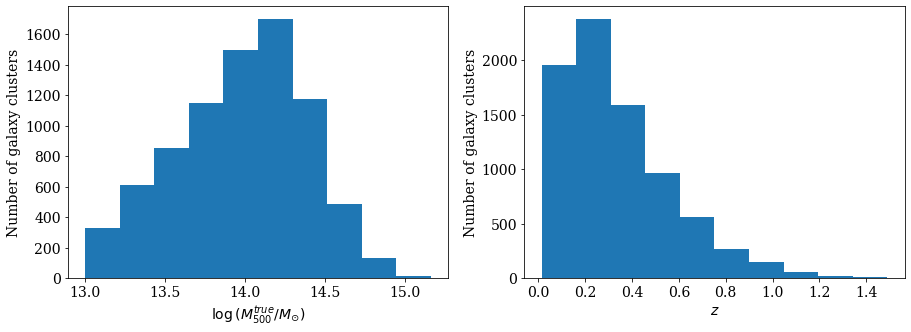
\includegraphics[width=\textwidth]{images/Chapter3/distr_data.png}
\caption{Distribution of the given galaxy cluster data. The mass distribution (\textit{left}) is roughly a normal distribution with a slight shift towards higher masses. The redshift (\textit{right}) is highly shifted towards smaller redshifts, meaning there are way more galaxy clusters with a shorter distance to Earth than clusters with greater distances.} 
\label{fig:data_dist}
\end{figure}

The actual galaxy cluster images do vary quite a bit in appearance. While there are galaxy clusters with a very obvious round or elliptical form (see \autoref{fig:cluster_big}), there are also clusters that are barely distinguishable from the background noise (see \autoref{fig:cluster_small}). In most cases the latter are either very small or far away while the opposite is true for galaxy clusters easily detectable with human-eye.

\begin{figure}[H]
\centering
\begin{subfigure}{.4\textwidth}
  \centering
  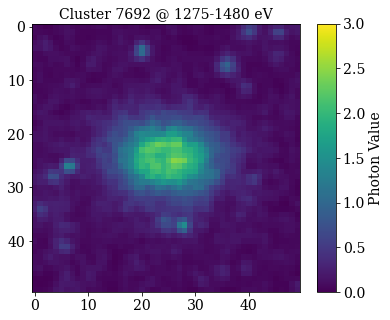
\includegraphics[width=\linewidth]{images/Chapter3/cluster_big.png}
  \caption{Galaxy cluster with a mass of $\log{(M_{500}^{\text{true}}/M_{\odot})} \approx 14.82$ at a redshift of $z \approx 0.12$}
  \label{fig:cluster_big}
\end{subfigure}%
\hspace{3.6em}
\begin{subfigure}{.4\textwidth}
  \centering
  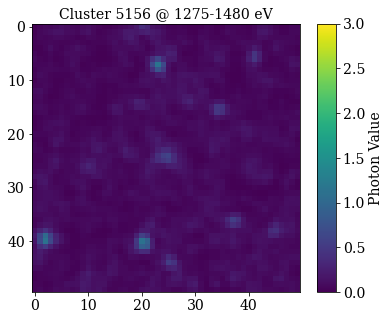
\includegraphics[width=\linewidth]{images/Chapter3/cluster_small.png}
  \caption{Galaxy cluster with a mass of $\log{(M_{500}^{\text{true}}/M_{\odot})} \approx 14.18$ at a redshift of $z \approx 0.3$}
  \label{fig:cluster_small}
\end{subfigure}
\caption{Two very different looking galaxy clusters at the same frequency band of $1275-1480 \text{eV}$ from the eFEDS simulation catalogue. The photon value is capped at three for easier visualisation.} 
\label{fig:cluster_comp}
\end{figure}


\begin{figure}[H]

\subfloat{%
  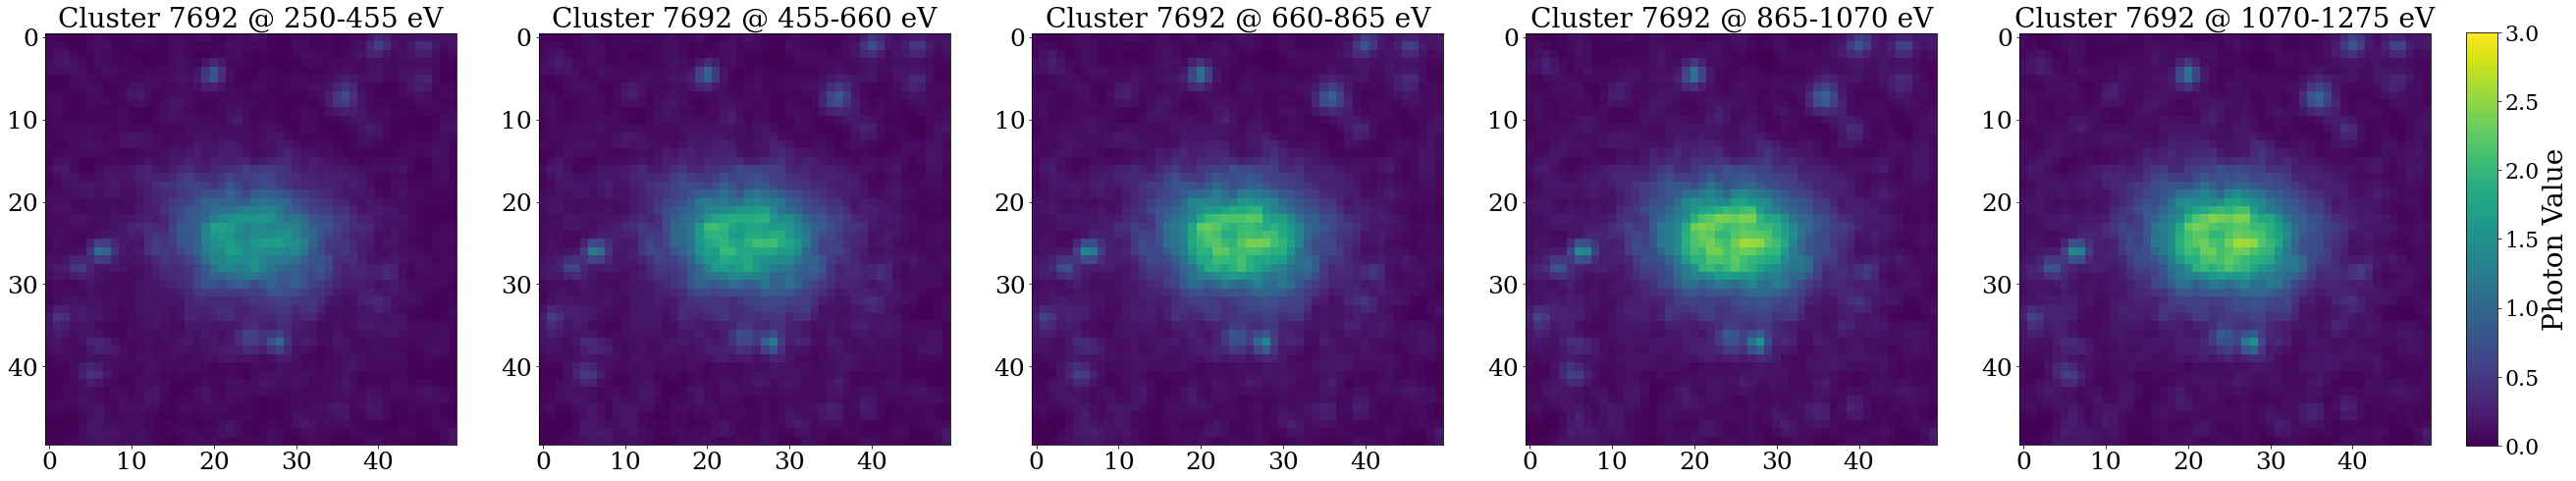
\includegraphics[clip,width=\columnwidth]{images/Chapter3/cluster_7692.png}%
}
\vspace{1em}
\subfloat{%
  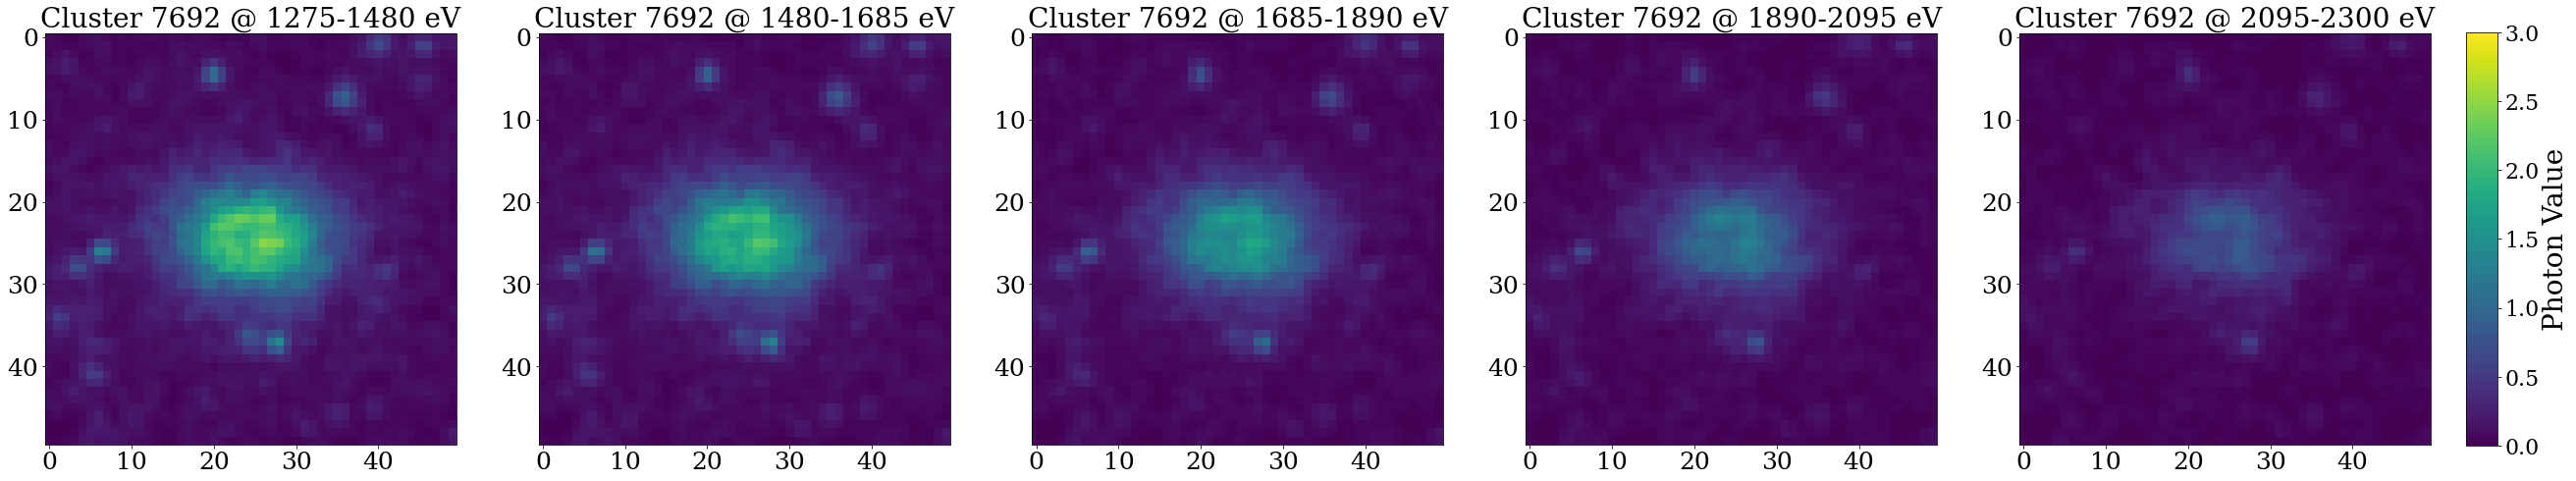
\includegraphics[clip,width=\columnwidth]{images/Chapter3/cluster_7692_II.png}%
}

\caption{All ten frequency bands for the galaxy from \autoref{fig:cluster_big}. Especially for higher frequencies, less photons are captured. Because of this, only frequencies up to $2300\text{eV}$ are being considered for mass estimation.}
\label{fig:cluster_big_freq}

\end{figure}
